\part{Appendix}
% !TeX root = ../main.tex
\section{Aalborg Tekniske Gymnasium Student and Teacher Interview (In danish)}
\label{Interviews1}
Projektstyring:
Analog og digital teknik.
Programmerbar teknologi.
Næsten ingen programmering i faget.
Allerede har haft programmering: Visual basic og C++
- B-niveau: Variabler, typer, kontrolstrukturer. 


Projekter:
- Cykellygte,
- Spilprojekt på arduino,
- Motor (Robot),
- Censorprojektet,
- Eksamensprojekt.

Spørgsmål: 
- Lave en funktion (opbygning)
- Lang tid på fejlsøgning.

Snakker meget for visuel programmering.
Giver forståelse for de initielle aspekter.


- Semikolon: Måske - (Men ja)
- Typer: Brug begge dele.
- Static vs dynamic typed: Så længe det virker. 
(Fare for at gøre noget uhensigtsmæssigt)

Faget: Ikke så meget forstå - mere bare lave.
 - Mindre fysik.

Er kurset i høj kurs: Har haft programmering -> vælger dette fag.

Digital design og udvikling (nyt fag, apps, spil, robotdesign)

Nogle skifter hurtigt. 
Andre har ingen erfaring, men vokser med opgaven.

Generelle hjælpelinjer:
- Nem tilkobling og interaktion med hw.

GPIO: LED - DC Motor. 
Nogle sensorer. 
Bluetooth.

Duden er hw fan.

=================================

Til elever:

Lidt C{\#} -> Programmering (C{\#})
Meget C{\#}
Godt lide computere, men programmering for "boxed" - Ikke skrive forkert. 
"Hyggeligt når det fungere"
Slet ingen programmering.
Opnået en del interesse igennem faget.
Linjefag. 
Alle har haft C{\#}.
Linjefag. 
C{\#} Programmering.
En rimelige skarp i javascript.

Programmering:
- Rigtige funtkionskald,
- Semikolon er fint - Det er okay (MEN PISSE TRÆLS NÅR MAN GLEMMER)
- Arrays - 0-indexed forvirrende - arrays forvirrende.
- Var ikke brugt. 
-> auto brugt.
- Kender ikke funktionskald (Mange forskellige)
- Problemer med typer - (Type inference ville være nemmere) - Men kan godt lide eksplicit type.
- Semikolon ikke træls - Skulle være.
- Aner intet om typer 
- Ikke problemer med typer.
- C{\#} Let at gå til -> IDE'en. 
- C vs C{\#} i ide -> De mener at det ville være lige svært i en almindelig text editor.
- Loops var svære. 
Forskel på loops.
- Kunne ikke se pointe med metoder.
- Nemmere uden typer. 
Lidt svært at lære typer.
- Svært ikke at lære typer til start?
- Synes det var fint ikke at forholde sig til typer i start (brugte lua)
- Meget udenadslære, ikke tænke sig til hvilke kommandoer der gør hvad. 
Det kunne være bedre fra IDE'en.
- Loops er forvirrende. 
"For"-navnet er ikke intuitivt. 
- En med JS synes godt med var.
- Lang tid på at lære typerne.
- Kunne samle tal typer til num.

Hvad kunne være bedre?: 
- Dokumentationen kunne være bedre.
- Man er vant til overhead -> Så det okay, men lidt tvilende. 
Men de mener også det er fordi det er det de har lært, og det nok kunne være simplere for begyndere.
- Error beskeder lort.
- Smart med ikke include.
- Kan ikke huske hvordan man laver funktion, men de siger det altid nemt at se hvordan man gjorde sidst.
- Bedre dokumentation
- Overflod af metoder.
- Eksempler til sproget.
- Lidt problemer med header og includes.
- Scoping er lidt svært.
- Nem tilgang til muligt funktions kald.
- Godt med afgrænsning fra {}
- En forslår indentation som fra python.

Arduino platformen:
- Den er fin, IDE dårlig ikke hjælper.
- Minestorm forturkket af en der er "Dårlig" til programmering.
- Love it. 
Det er simpelt.
- Arduino er "Dum" gør hvad den bliver bedt om -> godt.
- Svært med for mange komponenter, men generelt god læringsplatform.
- Godt med hands-on experience. 
Bedre med noget fysisk, end bare en terminal fra C{\#}.
- Svært med hvad forskellige gpio og ports gør.
- Ideen med at man får noget til at "Lyse" er fed!
- Fejlbeskeder er dårlige.
- Editoren burde hjælpe mere.


Læse videre:
- Software
- Nanoteknologi
- Maskinmester
- Programmering (Presset mod det.)
- Datalog 
- Bedre sprog kunne have øget interesse.
- Maskinmester
- En ville lave hjemmesider, men synes programmering ikke var underholdende, fordi læringskurve var for stejl.
- Vil gerne hurtigere nå målet.
- Sidste gruppe snakker rigtig meget for at et nemmere sprog kunne have øget interessen, og at de er blevet skræmt lidt væk.
- En software ingeniør. 


- Vores sprog: 
- Ikke så synligt for dem. 
Men efter forklaring gav mening.

- Første 3 gik meget hurtigt og klar igennem, 4 var lidt mere besværlig. 
Hjalp med parenteser.

- Gruppe løste alle 4 opgaver.
(Denne gruppe havde IKKE programmeret før)

- Denne gruppe acede det. 
Stadig en smule problemer med associering.

- Sidste gruppe var rimelig god, men stadig lidt tvivl om associering.
\section{NPDA for HCL}
\label{NPDA}
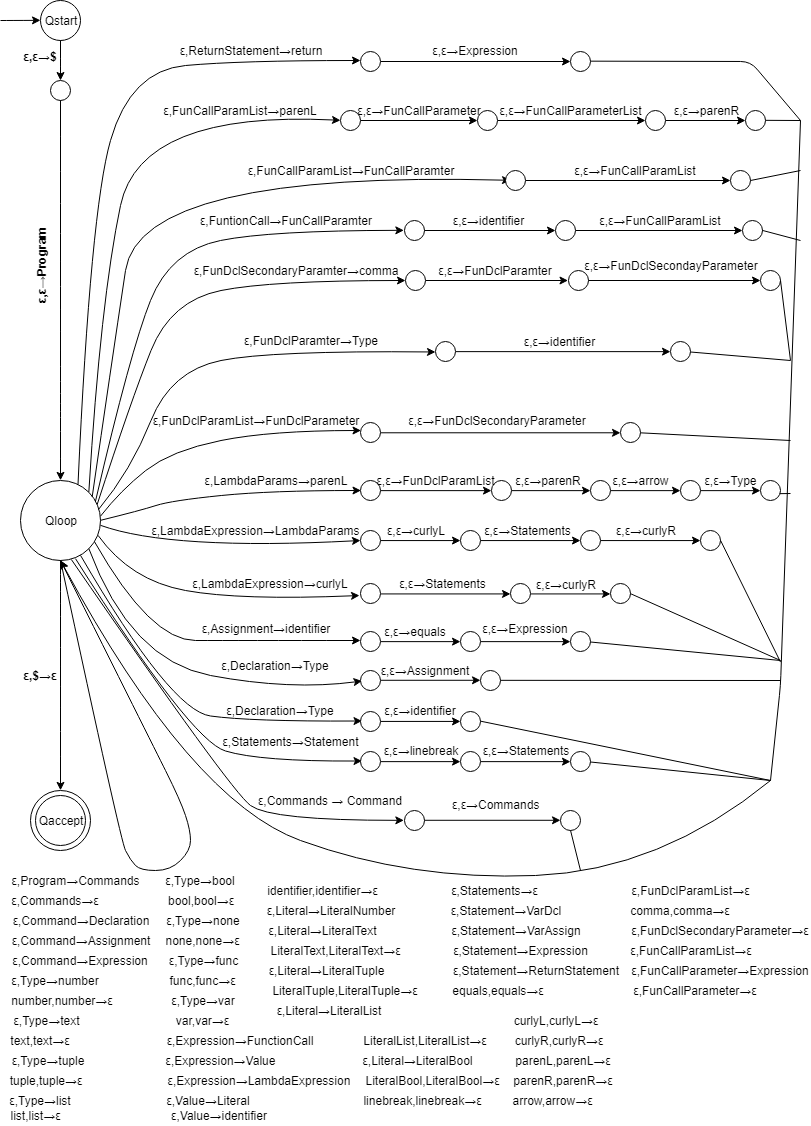
\includegraphics[width=\textwidth]{Appendix/images/NPDA.png}

\section{Aalborg Tekniske Gymnasium Student and Teacher Interview (In danish)}
\label{Interviews}
Projektstyring
Analog og digital teknik.
Programmerbar teknologi.
Næsten ingen programmering i faget.
Allerede har haft programmering: Visual basic og C++
- B-niveau: Variabler, typer, kontrolstrukturer. 


Projekter:
- Cykellygte,
- Spilprojekt på arduino,
- Motor (Robot),
- Censorprojektet,
- Eksamensprojekt.

Spørgsmål: 
- Lave en funktion (opbygning)
- Lang tid på fejlsøgning.

Snakker meget for visuel programmering.
Giver forståelse for de initielle aspekter.


- Semikolon: Måske - (Men ja)
- Typer: Brug begge dele.
- Static vs dynamic typed: Så længe det virker. (Fare for at gøre noget uhensigtsmæssigt.)

Faget: Ikke så meget forstå - mere bare lave. - Mindre fysik.

Er kurset i høj kurs: Har haft programmering -> vælger dette fag.

Digital design og udvikling (nyt fag, apps, spil, robotdesign)

Nogle skifter hurtigt. Andre har ingen erfaring, men vokser med opgaven.

Generelle hjælpelinjer:
- Nem tilkobling og interaktion med hw.

GPIO: LED - DC Motor. Nogle sensorer. Bluetooth.

Duden er hw fan.

=================================

Til elever:

Lidt C{\#} -> Programmering (C{\#})
Meget C{\#}
Godt lide computere, men programmering for "boxed" - Ikke skrive forkert. 
"Hyggeligt når det fungere"
Slet ingen programmering.
Opnået en del interesse igennem faget.
Linjefag. Alle har haft C{\#}.
Linjefag. C{\#} Programmering.
En rimelige skarp i javascript.

Programmering:
- Rigtige funtkionskald,
- Semikolon er fint - Det er okay (MEN PISSE TRÆLS NÅR MAN GLEMMER.)
- Arrays - 0-indexed forvirrende - arrays forvirrende.
- Var ikke brugt. -> auto brugt.
- Kender ikke funktionskald (Mange forskellige)
- Problemer med typer - (Type inference ville være nemmere) - Men kan godt lide eksplicit type.
- Semikolon ikke træls - Skulle være.
- Aner intet om typer 
- Ikke problemer med typer.
- C{\#} Let at gå til -> IDE'en. 
- C vs C{\#} i ide -> De mener at det ville være lige svært i en almindelig text editor.
- Loops var svære. Forskel på loops.
- Kunne ikke se pointe med metoder.
- Nemmere uden typer. Lidt svært at lære typer.
- Svært ikke at lære typer til start?
- Synes det var fint ikke at forholde sig til typer i start (brugte lua)
- Meget udenadslære, ikke tænke sig til hvilke kommandoer der gør hvad. Det kunne være bedre fra IDE'en.
- Loops er forvirrende. "For"-navnet er ikke intuitivt. 
- En med JS synes godt med var.
- Lang tid på at lære typerne.
- Kunne samle tal typer til num.

Hvad kunne være bedre?: 
- Dokumentationen kunne være bedre.
- Man er vant til overhead -> Så det okay, men lidt tvilende. Men de mener også det er fordi det er det de har lært, og det nok kunne være simplere for begyndere.
- Error beskeder lort.
- Smart med ikke include.
- Kan ikke huske hvordan man laver funktion, men de siger det altid nemt at se hvordan man gjorde sidst.
- Bedre dokumentation
- Overflod af metoder.
- Eksempler til sproget.
- Lidt problemer med header og includes.
- Scoping er lidt svært.
- Nem tilgang til muligt funktions kald.
- Godt med afgrænsning fra {}
- En forslår indentation som fra python.

Arduino platformen:
- Den er fin, IDE dårlig ikke hjælper.
- Minestorm forturkket af en der er "Dårlig" til programmering.
- Love it. Det er simpelt.
- Arduino er "Dum" gør hvad den bliver bedt om -> godt.
- Svært med for mange komponenter, men generelt god læringsplatform.
- Godt med hands-on experience. Bedre med noget fysisk, end bare en terminal fra C{\#}.
- Svært med hvad forskellige gpio og ports gør.
- Ideen med at man får noget til at "Lyse" er fed!
- Fejlbeskeder er dårlige.
- Editoren burde hjælpe mere.


Læse videre:
- Software
- Nanoteknologi
- Maskinmester
- Programmering (Presset mod det.)
- Datalog 
- Bedre sprog kunne have øget interesse.
- Maskinmester
- En ville lave hjemmesider, men synes programmering ikke var underholdende, fordi læringskurve var for stejl.
- Vil gerne hurtigere nå målet.
- Sidste gruppe snakker rigtig meget for at et nemmere sprog kunne have øget interessen, og at de er blevet skræmt lidt væk.
- En software ingeniør. 


- Vores sprog: 
- Ikke så synligt for dem. Men efter forklaring gav mening.

- Første 3 gik meget hurtigt og klar igennem, 4 var lidt mere besværlig. Hjalp med parenteser.

- Gruppe løste alle 4 opgaver.(Denne gruppe havde IKKE programmeret før)

- Denne gruppe acede det. Stadig en smule problemer med associering.

- Sidste gruppe var rimelig god, men stadig lidt tvivl om associering.

\section{Extended Backus-Naur Form of HCL grammar}
\label{AppendixEBNF}
\begin{align*}
	\texttt{<Program>}\to & \texttt{ <Cmds> \$}\\
	\texttt{<Cmds>}\to & \texttt{ \{<Cmd>\}}\\
	\texttt{<Cmd>}\to & \texttt{ <VarDcl> linebreak}\\
	| & \texttt{ <Assign> linebreak}\\
	| & \texttt{ <Expr> linebreak}\\
	| & \texttt{ <ReturnCmd> linebreak}\\
	\texttt{<Dcl>}\to & \texttt{ <ImplicitType> identifier [equals <DclValue>]}\\
	\texttt{<ImplicitType>}\to & \texttt{ <Type>}\\
	| & \texttt{ func}\\
	| & \texttt{ var}\\
	\texttt{<Type>}\to & \texttt{ number}\\
	| & \texttt{ text}\\
	| & \texttt{ tuple sqBracketL [<TypeList>] sqBracketR}\\
	| & \texttt{ list sqBracketL [<Type>] sqBracketR}\\
	| & \texttt{ bool}\\
	| & \texttt{ func sqBracketL [<TypeListNoneAndGenerics>] sqBracketR}\\
	| & \texttt{ none}\\
	\texttt{<TypeList>}\to & \texttt{ <Type> [comma <TypeList>]}\\
	\texttt{<TypeListGenerics>}\to & \texttt{ <TypeGenerics> [separator <TypeListGenerics>] }\\
	\texttt{<TypeNoneAndGenerics>}\to & \texttt{<TypeGenerics>}\\
	| & \texttt{ none}\\
	\texttt{<TypeListNoneAndGenerics>} \to & \texttt{ <TypeNoneAndGenerics> [separator <TypeListNoneAndGenerics>]}\\
	\texttt{<TypeGenerics>}\to & \texttt{<Type>}\\
	| & \texttt{ identifier}\\
	\texttt{<Expr>}\to & \texttt{ <FunctionCall>}\\
	| & \texttt{ <Value>}\\
	| & \texttt{ parenL <Expr> parenR }\\
	\texttt{<Value>}\to & \texttt{ <Literal>}\\
	| & \texttt{ identifier}\\
	\texttt{<Literal>}\to & \texttt{ literalNumber}\\
	| & \texttt{ literalText}\\
	| & \texttt{ literalBool}\\
	| & \texttt{ <LiteralTuple>}\\
	| & \texttt{ <LiteralList>}\\
	\texttt{<Values>}\to & \texttt{ <Value> [comma <Values>]}\\
\end{align*} %pagebreak
\begin{align*}
	\texttt{<LiteralTuple>}\to & \texttt{ parenL <Values> parenR}\\
	\texttt{<LiteralList>}\to & \texttt{ sqBracketL <Values> sqBracketR}\\
	\texttt{<DclValue>}\to & \texttt{ <Expr>}\\
	| & \texttt{ <LambdaExpr>}\\
	\texttt{<Assign>}\to & \texttt{ identifier equals <DclValue>}\\
	\texttt{<LambdaExpr>}\to & \texttt{ parenL [<FunDclParams>] parenR colon <TypeNoneAndGenerics> {linebreak} <LambdaBody>}\\
	\texttt{<LambdaBody>}\to & \texttt{ curlyL <Cmds> curlyR}\\
	\texttt{<FunDclParams>}\to & \texttt{ <FunDclParam> [comma <FunDclParams>]}\\
	\texttt{<FunDclParam>}\to & \texttt{ <TypeListGenerics> identifier}\\
	\texttt{<FunctionCall>}\to & \texttt{ identifier}\\
	| & \texttt{ <Arg> identifier [<Args>]}\\
	\texttt{<Args>}\to & \texttt{ \{<Arg>\}+}\\
	| & \texttt{ parenL \{<Arg>\}+ parenR}\\
	\texttt{<Arg>}\to & \texttt{[colon]<Value>}\\
	| & \texttt{ <LambdaExpr>}\\
	| & \texttt{ <LambdaBody>}\\
	\texttt{<ReturnCmd>}\to & \texttt{ return <Expr>}
\end{align*}
\newpage
\section{HCL Built-In Functions}
\label{builtinAppend}
\textbf{Arithmetic Operations}\\
HCL includes five standard arithmetic functions for use on numerical values.
The functions are seen in table \ref{tbl:arith}.

\begin{table}[h]
	\centering
	\caption{Arithmetic Functions}
	\label{tbl:arith}
	\begin{tabular}{|c|c|c|c|}
		\hline
		Operation      & Symbol & Input Parameters & Return Type \\ \hline
		Addition       & +      & num, num         & num         \\ \hline
		Subtraction    & -      & num, num         & num         \\ \hline
		Division       & /      & num, num         & num         \\ \hline
		Multiplication & *      & num, num         & num         \\ \hline
		Modulo         & mod    & num, num         & num         \\ \hline
	\end{tabular}
\end{table}

\textbf{Boolean Operations}\\
Functions for boolean operations are listed in table \ref{tbl:bool}.
These functions compare numeral, textual or boolean values and returns a boolean value.

\begin{table}[h!]
	\centering
	\caption{Boolean Functions}
	\label{tbl:bool}
	\begin{tabular}{|c|c|c|c|}
		\hline
		Operation                                                       & Symbol         & Input Parameters & Return Type \\ \hline
		Smaller Than                                                    & \textless{}    & num, num         & bool        \\ \hline
		\begin{tabular}[c]{@{}c@{}}Smaller Than \\ Equals\end{tabular}  & lessThanEqual  & num, num         & bool        \\ \hline
		Greater Than                                                    & \textgreater{} & num, num         & bool        \\ \hline
		Numerical Equals                                                & equals         & num, num         & bool        \\ \hline
		\begin{tabular}[c]{@{}c@{}}Numerical Not \\ Equals\end{tabular} & notEquals      & num, num         & bool        \\ \hline
		And                                                             & and            & bool, bool       & bool        \\ \hline
		Or                                                              & or             & bool, bool       & bool        \\ \hline
		Textual Equals                                                  & equals         & txt, txt         & bool        \\ \hline
		\begin{tabular}[c]{@{}c@{}}Textual Not \\ Equals\end{tabular}   & notEquals      & txt, txt         & bool        \\ \hline
		Not                                                             & not            & bool             & bool        \\ \hline
	\end{tabular}
\end{table}
\newpage

\textbf{Text Manipulation}\\
Functions used to manipulate text-objects or converts values to text, seen in table \ref{tbl:text}.
\begin{table}[h!]
	\centering
	\caption{Textual Functions}
	\label{tbl:text}
	\begin{tabular}{|c|c|c|c|}
		\hline
		Operation       & Symbol & Input Parameters & Return Type \\ \hline
		Concat Text     & +      & txt, txt         & txt         \\ \hline
		Numeric To Text & toText & num              & txt         \\ \hline
		Boolean To Text & toText & bool             & txt         \\ \hline
		Textual To Text & toText & txt              & txt         \\ \hline
		List To Text    & toText & list{[}T{]}      & txt         \\ \hline
	\end{tabular}
\end{table}


\textbf{Control Structures}\\
Functions used as control structures in HCL, seen in table \ref{tbl:control}
\begin{table}[h]
	\centering
	\caption{Control Structures}
	\label{tbl:control}
	\begin{tabular}{|c|c|c|c|}
		\hline
		Operation                                                 & Symbol & Input Parameters            & Return Type \\ \hline
		\begin{tabular}[c]{@{}c@{}}Then \\ Statement\end{tabular} & then   & bool, func{[}none{]}        & bool        \\ \hline
		While Loop                                                & while  & func{[}none{]}, bool        & bool        \\ \hline
		Foreach Loop                                              & each   & list{[}T{]}, func{[}none{]} & none        \\ \hline
	\end{tabular}
\end{table}

\textbf{List Operations}\\
Functions used to manipulate or monitor lists, seen in table \ref{tbl:list}.
\begin{table}[h]
	\centering
	\caption{List Operations}
	\label{tbl:list}
	\begin{tabular}{|c|c|c|c|}
		\hline
		Operation     & Symbol  & Input Parameters            & Return Type \\ \hline
		Get Lenght    & lenght  & list{[}T{]}                 & num         \\ \hline
		At Index      & at      & list{[}T{]}, num            & T           \\ \hline
		Concatenation & +       & list{[}T{]}, List{[}T{]}    & list{[}T{]} \\ \hline
		Get Sublist   & subList & list{[}T{]}, num, num       & list{[}T{]} \\ \hline
		Map           & map     & list{[}T{]}, func[T, T]     & list{[}T{]} \\ \hline
		Filter List   & filter  & list{[}T{]}, func[T, bool]  & list{[}T{]} \\ \hline
	\end{tabular}
\end{table}
\newpage

\textbf{Pin-Functions}\\
Functions used to read and write from arduino's analogue and digital pins, seen in table \ref{tbl:pins}.
\begin{table}[h]
	\centering
	\caption{Pin Operations}
	\label{tbl:pins}
	\begin{tabular}{|c|c|c|c|}
		\hline
		Operation                                                      & Symbol         & Input Parameters & Return Type \\ \hline
		Set Digital Pin                                                & setDigitalPin  & num, bool        & none        \\ \hline
		Read Digital Pin                                               & readDigitalPin & num              & num         \\ \hline
		Write Analog Pin                                               & setAnalogPin   & num, num         & none        \\ \hline
		Read Analog Pin                                                & readAnalogPin  & num              & num         \\ \hline
		Delay                                                          & delayMillis    & num              & none        \\ \hline
	\end{tabular}
\end{table}

\textbf{Print Operations}\\
Functions used to print to output, seen in table \ref{tbl:print}.
\begin{table}[h]
	\centering
	\caption{Print Functions}
	\label{tbl:print}
	\begin{tabular}{|c|c|c|c|}
		\hline
		Operation  & Symbol    & Input Parameters & Return Type \\ \hline
		Print      & print     & num/bool/txt     & none        \\ \hline
		Print List & print     & list[T]          & none        \\ \hline
	\end{tabular}
\end{table}
\newpage
% !TeX root = ../main.tex
\begin{landscape}
\section{Semantics Derivation Tree Example}
\label{sec:semanticsTree}
This is an example of how to create a derivation tree for a program written in HCL.
It is based on the following code snippet.

\begin{lstlisting}[language=HCL,label=lis:derivationCode,firstnumber=1]
num x
x = 5
\end{lstlisting}

Rewritten using the abstract syntax described in section \ref{sec:semantics}, we get the following big step semantic:

\begin{center}
	$env_V, env_F \vdash \langle num\ x;\ x = 5, env_V, env_F, sto \rangle \rightarrow_{stm} (sto', env_V', env_F')$
\end{center}
Using the Compositional Big Step Semantic rule, the following derivation is produced:

\begin{center}
	\begin{math}
		\cfrac
		{env_V, env_F \vdash \langle num\ x, env_V, env_F, sto \rangle \rightarrow_{stm} (sto'', env_V'', env_F'')\quad env_V'', env_F'' \vdash \langle x = 5, env_V'', env_F'', sto'' \rangle \rightarrow_{stm} (sto', env_V', env_F')}
		{env_V, env_F \vdash \langle num\ x;\ x = 5, env_V, env_F, sto \rangle \rightarrow_{stm} (sto', env_V', env_F')}
	\end{math}
\end{center}

Table \ref{tbl:progstates} shows how the program state changes after each statement in the code is run.

\begin{table}[H]
	\centering
	\caption{Table of program states after each statement.}
	\label{tbl:progstates}
	\setlength\extrarowheight{5pt}
	\begin{tabular}{|c|c|c|}
		\hline
		& Abstract program state      & Concrete program state                          \\ \hline
		Initial state          & $(sto, env_V, env_F)$       & $(sto, env_V, env_F)$                           \\ \hline
		After first statement  & $(sto'', env_V'', env_F'')$ & $(sto[l \mapsto 0], env_V[x \mapsto l], env_F)$ \\ \hline
		After second statement & $(sto', env_V', env_F')$    & $(sto[l \mapsto 5], env_V[x \mapsto l], env_F)$  \\ \hline
	\end{tabular}
\end{table}

\end{landscape}
% !TeX root = ../main.tex
\section{Type Rule Derivation Tree Example}
\label{sec:typeRuleTree}
This is an example of how to create a type derivation tree for a program written in HCL. It is based on the following code snippet.

\begin{lstlisting}[language=HCL,label=lis:typeTreeCode]
num x = 5
bool b = x greaterThan 0
b print
\end{lstlisting}

The program calls two functions, $greaterThan$ and $print$.
They are declared with the following types:

\begin{lstlisting}[language=HCL,label=lis:typeTreeCode]
func[num, num, bool] greaterThan # Two number parameters, returns bool
func[bool, none] print # overloaded to take a bool parameter, returns nothing
\end{lstlisting}

Following the type rules specified in section \ref{typerules}, the derivation tree will look like this:
\begin{center}
	\begin{math}
		\cfrac
		{\cfrac
			{E\vdash 5 : num}
			{E\vdash num\ x = 5 : \texttt{ok}}\quad \cfrac
				{\cfrac
					{\cfrac
						{E(x) : num\quad E \vdash 0 : num}
						{E\vdash x\ greaterThan\ 0: bool}}
					{E\vdash bool\ b = x\ greaterThan\ 0 : \texttt{ok}}\quad \cfrac
					{E\vdash b : bool}
					{E\vdash b\ print : (none, \texttt{ok})}}
				{E\vdash bool\ b = x\ greaterThan\ 0;\ b\ print : \texttt{ok}}}
		{E \vdash num\ x = 5;\ bool\ b = x\ greaterThan\ 0;\ b\ print : \texttt{ok}}
	\end{math}
\end{center}
